\documentclass[a4paper,notitlepage]{report}
\usepackage[dutch]{babel}
\usepackage{mathtools}
\usepackage[dvipsnames]{xcolor}
\usepackage{amsfonts,amsmath,amstext,amssymb,caption,mathtools,tikz}
\usepackage{listings, float}
\captionsetup{width = 0.8\textwidth, font=small, textfont=it, labelfont=bf}
%
\addto\captionsdutch{%
  \def\lstlistingname{Programma}}
%
\usetikzlibrary{babel}
\usepackage[hidelinks]{hyperref}

\widowpenalty10000
\clubpenalty10000

\author{Benny Aalders \and Vincent Velthuizen}
\title{Voorbeelden van instructies voor docenten}
\date{\today}
%\newcommand\variable[1]{{\ttfamily\textless#1\textgreater}}
%\let\slash/
%\catcode`\/=13
%\def/{\slash\allowbreak}
\newcommand{\notitie}[3][*]{\underline{#2}#1\marginpar{\hspace{-1.3ex}#1\scriptsize#3}}
\setlength{\marginparwidth}{100pt}
\newcommand\ggd{\ensuremath{\operatorname{ggd}}}
\newcommand\kgv{\ensuremath{\operatorname{kgv}}}

\def\opdracht#1{%
\begin{tikzpicture}[baseline=(nodename.base)]
		 	\node[draw=opdrachtkleur,fill=opdrachtkleur,text=white] (nodename) {\bfseries #1};
		\end{tikzpicture}%
}

\definecolor{opdrachtkleur}{RGB}{204,0,0} %Initialiseer op RUG-rood
\definecolor{J1H2}{RGB}{204,102,0}
\definecolor{J2H6}{RGB}{132,133,255}
\definecolor{J3H5}{RGB}{175,0,175}

\lstset{
	keepspaces=true,
	frame=tBlR,
	rulesepcolor=\color{opdrachtkleur},
	numbers=left,
	tabsize=2,
	breaklines=true,
	breakatwhitespace=true,
	captionpos=b,
	postbreak={\mbox{$\cdots$}},
	prebreak={\mbox{$\cdots$}},
	mathescape=true,%
	}
	
\def\pijl{
	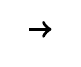
\begin{tikzpicture}[very thick,x=1em,y=1em,baseline={(0,-0.35em)}]
		\draw [->](-0.4,0) -- (0.4,0);
	\end{tikzpicture}
	}
\def\eindpijl{
	
\begin{tikzpicture}[very thick,x=1em,y=1em,baseline={(0,-0.3em)}]
		\draw[<-] (-0.25,0) -- (0.25,0) -- (0.25,0.3); 
	\end{tikzpicture}
	}
\def\vervolg{
	
\begin{tikzpicture}[very thick,x=1em,y=1em,baseline={(0,-0.3em)}]
		\draw[<-] (0.25,0) -- (-0.25,0) -- (-0.25,0.3); 
	\end{tikzpicture}%
	}
\def\dakje{
	
\begin{tikzpicture}[very thick,x=1em,y=1em,baseline={(0,0)}]
		\draw (-0.3,0.3) -- (0,0.7) -- (0.3,0.3);
	\end{tikzpicture}
	}
\def\dh{
	
\begin{tikzpicture}[very thick,x=1em,y=1em,baseline={(0,0)}]
		\filldraw (0,0) -- (0.3,0) -- (0.3,0.3) -- cycle;
	\end{tikzpicture}
	}
\def\sp{\bfseries\textvisiblespace}
\lstdefinestyle{basic}{%
	language=[Visual]Basic,%
	keywordstyle=\bfseries\underbar,%
	commentstyle=\itshape\small,%
	mathescape=true,%
	morekeywords={To,LpWhile,IfEnd,Step,Lbl,Locate,ClrText},%
	literate={->}{\pijl}1 {;}{\eindpijl}1{^}{\dakje}1{;;}{\dh}1%
	}
	
\lstdefinestyle{pascal}{%
	language=Pascal,
	keywordstyle=\bfseries\underbar,%
	commentstyle=\itshape\small,%
	mathescape=true,%
	deletekeywords=[1]{mod,false},%
	morekeywords={RETURN,EXPORT,LOCAL,FROM},
	morecomment=[l]{//},
}

\lstdefinelanguage{pseudo}
{
  % list of keywords
  morekeywords={invoer,uitvoer,voor,als,dan,anders,geef,print,zolang,zeg},
  sensitive=false, % keywords are not case-sensitive
  morecomment=[l]{//}, % l is for line comment
  morecomment=[s]{/*}{*/}, % s is for start and end delimiter
  morestring=[b]" % defines that strings are enclosed in double quotes
}

\def\lstsqrt#1{\raisebox{3pt}[\totalheight][0pt]{$\smash{\sqrt{#1}}$}}


\hyphenation{hulp-pro-gramma}

\renewcommand{\thesection}{\arabic{section}}
\begin{document}

\maketitle

\section{Doel van dit document}
Om te voldoen aan de eisen van het SLO met betrekking tot Digitale Geletterdheid moeten leerlingen bepaalde vaardigheden verwerven. Een deel van die vaardigheden worden in zekere mate al gedekt door het wiskundecurriculum. Dit document beschrijft hoe het leren en verifi\"eren van die vaardigheden expliciet te maken is. Het is de bedoeling zo min mogelijk af te wijken van de bestaande leerlijnen. Voor de leerlingen bestaat er een apart document. Dit document is opgesteld om gelijk te lopen met de gebruikte wiskunde methode.

In deze versie van het document zijn voor het begin, het midden en het einde van de onderbouw opdrachten opgenomen. Dit geeft een beeld van de verwachtingen die wij hebben van het niveau dat de leerlingen hebben en zullen verwerven gedurende deze periode.  Er is momenteel alleen een document voor de leerlingen beschikbaar dat hoort bij  de methode Getal \& Ruimte.

\section{Opbouw van dit document}

De hoofdtekst in dit document is bedoeld om de docent in staat te stellen de leerling te helpen bij het zelf verwerven van de vaardigheden. We geven voor ieder probleem een oplossing in pseudocode die deels of geheel aan de leerling kan worden aangeboden om hem of haar op weg te helpen. We geven ook aan waar veelvoorkomende fouten zitten. De opdrachten zelf geven aan welke testdata relevant zijn om de werking van het programma te verifi\"eren.

Het is aan de docent om te bepalen hoe de code beoordeeld moet worden. Onze suggestie is te streven naar werkende code (niet noodzakelijk mooie, elegante of effici\"ente code) en om de beoordeling te beperken tot voldoende/onvoldoende.

In de appendix zijn referentie-implementaties opgenomen voor de verschillende opdrachten. Deze implementaties dienen niet als antwoordmodel maar kunnen door de docent gebruikt worden om snel een goede oplossing op te kunnen zoeken om een leerling verder te helpen.

\section{Opdrachten HAVO/VWO}

\subsection{Jaar 1}
\colorlet{opdrachtkleur}{J1H2}

%\subsubsection{\ggd en \kgv}

De leerlingen zijn bezig geweest om de \ggd\ en het \kgv\ uit te rekenen. Dit doen ze  aan de hand van een stappenplan. De bedoeling is om een programma te schrijven dat hetzelfde stappenplan volgt. In pseudocode ziet dat er uit zoals in \autoref{pseudo:ggd}.

In opdrachten \opdracht{P1} en \opdracht{P2} moeten de leerlingen experimenteren met de (aangeleverde) functie isDeler?

In opdracht \opdracht{P3} moeten de leerlingen een lus gebruiken, dit is misschien nieuw. Merk op dat dit een FOR lus dient te zijn, aangezien het aantal iteraties bekend is. Merk ook op dat elk getal een deler is van zichzelf. Een slimme eindconditie (bijvoorbeeld getal/2) dient daar rekening mee te houden.

De extra moeilijkheid in \opdracht{P4} is het handig doorlopen van de lijsten die ze maken (die lijsten maken is een kwestie van het kopi\"{e}ren/plakken van de code uit \opdracht{P3}). De leerling zou onderaan de lijst kunnen beginnen waardoor juist de kleinste gemene deler wordt gevonden. Ook het bedenken voor welke lijst de iterator verlaagd moet worden, vereist enig inzicht. Mochten veel leerlingen moeite hebben bij deze opdracht dan kan het tekenen van de lijsten op het bord, met waardes en indices een waardevolle tussenstap zijn.

\begin{lstlisting}[language=pseudo, caption={Pseudocode voor \ggd}, label={pseudo:ggd}]
ggd
invoer : A, B
uitvoer: GGD

voor elk GETAL tussen 1 en A
	als GETAL een deler van A is
		voeg GETAL toe aan DELERS_A
		
voor elk GETAL tussen 1 en B
	als het GETAL een deler van B is
		voeg GETAL toe aan DELERS_B
		
begin onder aan lijsten DELERS_A en DELERS_B
	als de waardes gelijk zijn
		geef GGD
	als de waarde uit DELERS_A groter dan die uit DELERS_B is
		ga 1 omhoog in de lijst DELERS_A
	als de waarde uit DELERS_A kleiner dan die uit DELERS_B is
		ga 1 omhoog in de lijst DELERS_B
\end{lstlisting}

Bij opdracht \opdracht{P7} moeten de leerlingen zich realiseren dat deze lijst geen einde heeft. Dit is ook het grootste risico voor fouten in de code (oneindige lus). Mocht een leerling een oneindige lus cre\"{e}ren, laat hem of haar dan in elke iteratie van de lus iets printen. Dit zal ze helpen te beseffen wat er aan de hand is. Help ze doen inzien dat  A $*$ B altijd een gemeen veelvoud is, en dat daar voorbij zoeken dus niet nodig is.

Opdracht \opdracht{P8} is vergelijkbaar met \opdracht{P4}. Het kan de moeite waard zijn om leerlingen te wijzen op de overeenkomsten mochten ze er niet uitkomen. De leerlingen die er wel uitkomen wordt gevraagd hierover na te denken in vraag \opdracht{P11}.

Opdracht \opdracht{P12} is vooral bedoeld om de snelle leerlingen iets te doen te geven. Het maken van een goede gebruikersinterface is belangrijk maar daar dient deze les niet voor.


\begin{lstlisting}[language=pseudo, caption={Pseudocode voor \kgv}, label={pseudo:kgv}]
kgv
invoer : A, B
uitvoer: KGV

voor elk GETAL tussen 1 en B
	voeg GETAL * A toe aan VEELVOUDEN_A
		
voor elk GETAL tussen 1 en A
	voeg GETAL * B toe aan VEELVOUDEN_B
		
begin boven aan lijsten VEELVOUDEN_A en VEELVOUDEN_B
	als de waardes gelijk zijn
		geef KGV
	als de waarde uit DELERS_A kleiner dan die uit DELERS_B is
		ga 1 omlaag in de lijst DELERS_A
	als de waarde uit DELERS_A kleiner dan die uit DELERS_B is
		ga 1 omlaag in de lijst DELERS_B
\end{lstlisting}

\clearpage
\subsection{Jaar 2}
\colorlet{opdrachtkleur}{J2H6}

\subsubsection{Gemiddelde, Mediaan en Modus}

De leerlingen moeten een lijst kunnen laden om deze opdrachten op uit te voeren (\opdracht{P13\textbf{a}}). Het kan zijn dat de leerlingen wat hulp nodig hebben om in te zien dat een lijst bestaande uit meerdere elementen toch \'e\'en parameter kan zijn. Het is belangrijk dat de leerlingen het itereren over een lijst goed onder de knie krijgen dat gaan ze dit hoofdstuk uitgebreid nodig hebben en oefenen.

\begin{lstlisting}[language=pseudo, caption={Pseudocode voor gemiddelde}, label={pseudo:gemiddelde}]
gemiddelde
invoer : LIJST
uitvoer: de gemiddelde waarde van de lijst

voor elke waarde in LIJST
	tel op bij SOM

GEMIDDELDE is SOM gedeeld door het aantal elementen in de lijst
geef GEMIDDELDE
\end{lstlisting}

De leerlingen moeten eerst een aantal hulpfuncties implementeren (\opdracht{P14}, \opdracht{P15}, \opdracht{P16\textbf{(a,b,c)}}. Het schrijven en vervolgens gebruiken van de hulpfuncties zou ze moeten stimuleren in toekomstige opdrachten te kijken of er nuttige bestaande functies zijn die ze kunnen (her)gebruiken.

In opdracht \opdracht{P16\textbf{(d, e, f)}} schrijven ze vervolgens de code voor het vinden van de mediaan, en het testen van dat programma.

\begin{lstlisting}[language=pseudo, caption={Pseudocode voor max}, label={pseudo:max}]
max
invoer : LIJST
uitvoer: MAX

MAX := eerste waarde uit de lijst
voor elk GETAL in LIJST (behalve de eerste)
	is GETAL groter dan MAX?
		MAX := GETAL
geef MAX 
\end{lstlisting}

\begin{lstlisting}[language=pseudo, caption={Pseudocode voor mindex}, label={pseudo:mindex}]
mindex
invoer : LIJST
uitvoer: GETAL (van het kleinste getal uit LIJST)

MIN := eerste waarde uit LIJST
INDEX := INDEX van de eerste waarde uit LIJST (vaak 0 of 1)
voor elk GETAL in LIJST (behalve de eerste)
	is GETAL kleiner dan MIN?
		MIN := GETAL
		INDEX := huidige index in de lijst
geef INDEX
\end{lstlisting}

\begin{lstlisting}[language=pseudo, caption={Pseudocode voor sort}, label={pseudo:sort}]
sort
invoer : LIJST
uitvoer: GESORTEERDE_LIJST

zolang LIJST niet leeg is
	voeg de kleinste waarde van LIJST toe aan GESORTEERDE_LIJST
	verwijder die waarde uit LIJST
	
geef GESORTEERDE_LIJST
\end{lstlisting}

\begin{lstlisting}[language=pseudo, caption={Pseudocode voor mediaan}, label={pseudo:mediaan}]
mediaan
invoer : LIJST
uitvoer: MEDIAAN

sorteer LIJST
is het aantal elementen in de lijst even?
	tel de middelste 2 bij elkaar en deel door twee; dit is de mediaan
	geef MEDIAAN
anders
	de middelste waarde is de mediaan
	geef MEDIAAN
\end{lstlisting}

Een algoritme voor het vinden van de modus wordt in het boek niet gegeven. We willen de leerlingen uitdagen zelf over een algoritme na te denken maar verwachten dat dit nog een flinke uitdaging kan zijn. In opdracht \opdracht{P17} dagen we ze uit hierover na te denken. We verwachten dat dit onderwerp zich goed leent om klassikaal te behandelen. Hierbij kan het ``denken'' van de computer op het bord uitgeschreven worden en kan de klas collectief nadenken over de te zetten stappen.

Een punt van aandacht is ook de definitie van modus. Volgens het boek zijn er 0 of 1 modi (als er meerdere zijn dan heeft de lijst volgens het boek geen modus). Het is, voor het door ons voorgestelde algoritme, beter als de leerlingen accepteren dat een lijst wel meerdere modi kan hebben.

\begin{lstlisting}[language=pseudo, caption={Pseudocode voor modus}, label={pseudo:modus}]
modus
invoer : LIJST
uitvoer: MODI

sorteer LIJST
houd bij:
welk getal tot nu toe het meest voor kwam, hoe vaak dat was
met welk getal je bezig bent, hoe vaak je die hebt gezien

voor elk GETAL in LIJST
	is dit het getal waar je nu mee bezig bent?
		aantal voorkomens van dit getal + 1
		is het aantal voorkomens nu groter dan het vorige maximum?
			dit getal is het nieuwe maximum, dit aantal voorkomens is het nieuwe maximum aantal voorkomens
		is dit aantal voorkomens gelijk aan het vorige maximum?
			dit getal is ook een modus voeg het toe aan de lijst van modi, het maximum aantal voorkomens blijft gelijk
	anders
		het getal waar je nu mee bezig bent is het getal uit de lijst
		het aantal voorkomens is 1
		is dit aantal voorkomens gelijk aan het vorige maximum?
			dit getal is ook een modus voeg het toe aan de lijst van modi, het maximum aantal voorkomens blijft gelijk

geef MODI
\end{lstlisting}

\clearpage
\subsection{Jaar 3}
\colorlet{opdrachtkleur}{J3H5}

De code voor de $abc$-formule is redelijk recht-toe-recht-aan. We  verwachten dat de leerlingen (met inmiddels 3 jaar programmeer ervaring) hier wel uit zouden moeten komen.

\subsubsection{$abc$-Formule}
\begin{lstlisting}[language=pseudo, caption={Pseudocode voor $abc$-formule}, label={pseudo:abc}]
abc
invoer : 
uitvoer: 
vraag de gebruiker om A, B, C in de formule ax^2+bx+c

DISCRIMINANT is B*B-4*A*C

als DISCRIMINANT kleiner dan 0 is
	zeg: er zijn geen oplossingen
anders, als de discriminant 0 is
	zeg: er is 1 oplossing
	OPLOSSING is (-B)/(2*A)
	geef OPLOSSING
anders
	zeg: er zijn 2 oplossingen
	EERSTE_OPLOSSING is (-B - wortel(discriminant))/(2*A)
	TWEEDE_OPLOSSING is (-B + wortel(discriminant))/(2*A)
	zeg: Xl=EERSTE_OPLOSSING, Xr=TWEEDE_OPLOSSING
\end{lstlisting}

\appendix\setlength{\parindent}{0mm}
\chapter*{Appendix}
\renewcommand{\thesection}{\Alph{section}}
\section{De \ggd\ en het \kgv}
\colorlet{opdrachtkleur}{J1H2}
\lstinputlisting[style=pascal, caption={Script van het programma isDeler, geschreven in HPPL.}]{./HP-Prime-Materiaal/Content/Jaar1/H2/isdeler.txt}

\lstinputlisting[style=pascal, caption={Script voor het berekenen van de \ggd\, geschreven in HPPL.}]{./HP-Prime-Materiaal/Content/Jaar1/H2/ggd.txt}

Merk op dat er in het KGV programma (\autoref{listing:kgv}) nog ``hulp'' uitvoer staat (regels \ref{lst:kgv:hulp1}, \ref{lst:kgv:hulp2} en \ref{lst:kgv:hulp3}) om de werking van het programma te zien. Het kan de leerlingen helpen inzicht te krijgen in hoe het programma werkt (en de computer ``denkt'') om zulke uitvoer te kunnen bestuderen.

\lstinputlisting[style=pascal, label={listing:kgv}, caption={Script voor het berekenen van het \kgv, geschreven in HPPL.}]{./HP-Prime-Materiaal/Content/Jaar1/H2/kgv.txt}

\autoref{listing:ggd_euclid} en \autoref{listing:kgv_euclid} laten effici\"{e}nte varianten van de programma's zien. Ze gebruiken het algoritme van Euclides. Het bewijs hiervan zal waarschijnlijk nog niet in het bereik van deze leerlingen liggen.

\lstinputlisting[style=pascal, label={listing:ggd_euclid}, caption={Effici\"ent script voor het berekenen van de \ggd, geschreven in HPPL.}]{./HP-Prime-Materiaal/Content/Jaar1/H2/ggd_euclid.txt}

\lstinputlisting[style=pascal, label={listing:kgv_euclid}, caption={Effici\"ent script voor het berekenen van het \kgv, geschreven in HPPL.}]{./HP-Prime-Materiaal/Content/Jaar1/H2/kgv_euclid.txt}

\section{Centrummaten}
\colorlet{opdrachtkleur}{J2H6}

\lstinputlisting[style=pascal, caption={Script voor het vinden van de maximale waarde in een lijst, geschreven in HPPL.}]{./HP-Prime-Materiaal/Content/Jaar2/H6/MAX.txt}

\lstinputlisting[style=pascal, caption={Script voor het vinden van de index van de minimale waarde in een lijst, geschreven in HPPL.}]{./HP-Prime-Materiaal/Content/Jaar2/H6/MINDEX.txt}

\lstinputlisting[style=pascal, caption={Na\"{i}ef script voor het sorteren van een lijst, geschreven in HPPL.}]{./HP-Prime-Materiaal/Content/Jaar2/H6/SORT.txt}

\lstinputlisting[style=pascal, caption={Script voor het berekenen van het gemiddelde van een lijst, geschreven in HPPL.}]{./HP-Prime-Materiaal/Content/Jaar2/H6/MEAN.txt}

\lstinputlisting[style=pascal, caption={Script voor het berekenen van de mediaan van een lijst, geschreven in HPPL.}]{./HP-Prime-Materiaal/Content/Jaar2/H6/MEDIAN.txt}

\bigskip
\lstinputlisting[style=pascal, caption={Script voor het berekenen van de modus (of modi) van een lijst, geschreven in HPPL.}]{./HP-Prime-Materiaal/Content/Jaar2/H6/MODE.txt}

\lstinputlisting[style=pascal, caption={Script voor het geven van een aantal statistieken van een lijst, geschreven in HPPL.}]{./HP-Prime-Materiaal/Content/Jaar2/H6/STATS.txt}

\section{De $abc$-formule}
\colorlet{opdrachtkleur}{J3H5}

\lstinputlisting[style=pascal, caption={Script voor het oplossen  van $ax^2+bx+c=0 $(over $\mathbb R$), geschreven in HPPL.}]{./HP-Prime-Materiaal/Content/Jaar3/ABCD/ABCD.txt}

\end{document}